\chapter{Molecular Biology}
Here in this chapter, I will be covering the basics of the relevant molecular biology concepts. This chapter will serve as a reference for the biological claims throughout the document, as well as the foundation for the review chapters of my thesis.

\section{Molecular Mechanism of Angiogenesis}

Blood vessels and the vascular structure are formed by the differentiation of the cells in the mesoderm layer during the embryo development (the layer which also give rise to blood cells, kidney, liver, connective tissue, etc.) \cite{Alberts2002}.

\subsection{A Brief Anatomy of Vessels}
Endothelial cells line all of the vessels. Blood vessels (like the arteries and the veins that are the largest vessels of the body) have a thick and tough wall of connective tissue with several layers of smooth muscles. The wall is lined by a very thin layer of endothelial cells (i.e. the endothelium) separated from the outer surrounding layers by basal lamina \cite{Alberts2002}. It is worth noting that the amount of connective tissue and smooth muscle depends on the diameter of the blood vessel as well as its function, \textbf{but the endothelial lining is always present}. In the finest branches of the vasculature (i.e. capillaries and sinusoids) the wall is just made up of endothelial cells and basal lamina. One of the major roles of the endothelial cells is to control to transport of material in an out of the bloodstream.

A study of embryo development reveals that the even larger vessels (like arteries and veins) start developing from smaller vessels that has only endothelial cells and basal lamina. The connective tissue, smooth muscles and pericytes are added later on, by the signaling from endothelial cells. In particular, the recruitment of pericytes are driven by PDGF (platelet driven growth factor) secreted by the endothelial cells.




\begin{figure}[h!]
	\centering
	% First bottom figure, occupying the left half
	\begin{minipage}{0.4\textwidth}
		\centering
		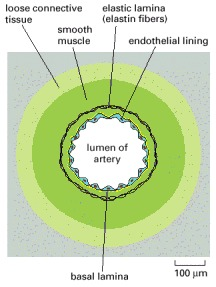
\includegraphics[width=\textwidth]{images/AnatomyOfVessel.jpg}
		% Optional caption for the first bottom image
		% \caption{Caption for the first bottom image.}
		% \label{fig:bottom-left-image}
	\end{minipage} % Space between the two bottom figures
	% Second bottom figure, occupying the right half
	\begin{minipage}{0.4\textwidth}
		\centering
		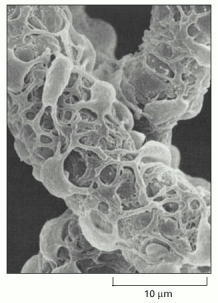
\includegraphics[width=\textwidth]{images/perycitesForVascular.jpg}
		% Optional caption for the second bottom image
		% \caption{Caption for the second bottom image.}
		% \label{fig:bottom-right-image}
	\end{minipage}
\end{figure}
\vspace{-15pt}
\begin{figure}[h!]
	% Top figure spanning the whole width
	\centering
	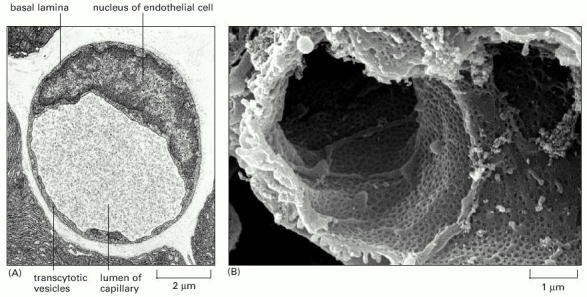
\includegraphics[width=0.8\textwidth]{images/ElectronMicroscopeOfVessel.jpg}
	% Optional caption for the top image
	\caption{\textbf{Figure Top Left:} This figure shows the anatomy of a large vessel, like vein or arteries. Note that smaller vessels, like capillaries as well as sinusoids consists of only endothelial cells and basal lamina, except for some scattered pericytes wrapped around the walls (see figure Top Left). \textbf{Figure Top Right:} Electron micro graph showing small pericytes wrapped around small blood vessels. \textbf{Figure Bottom Left:} A capillary that its wall consists of only endothelial cell and basal lamina. \textbf{Figure Bottom Right:} Electron micro graph showing a cross section of small capillary in pancreas. All of the figures are from \cite{Alberts2002}}

\end{figure}
\FloatBarrier

Also, the following figure summarizes the cross section of different types of vasculature.
\begin{figure}[h!]
	\centering
	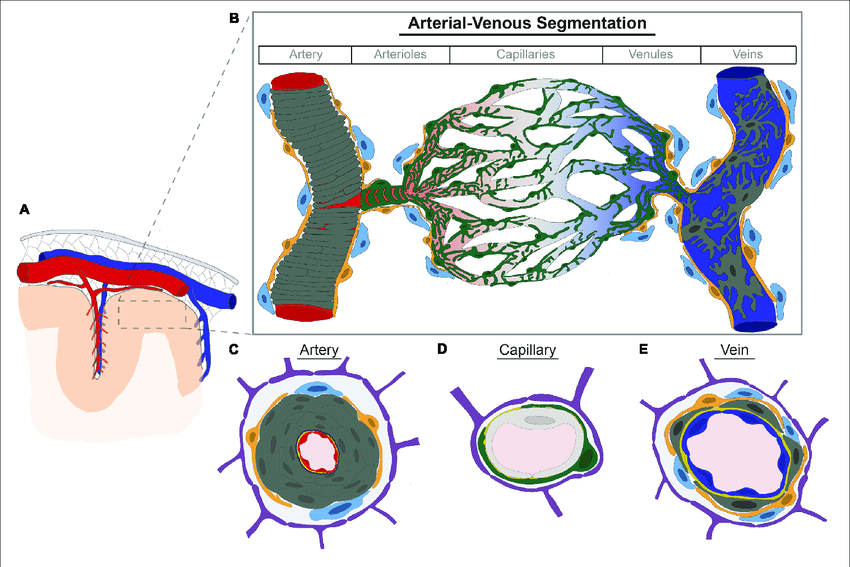
\includegraphics[width=0.8\textwidth]{images/CrossSectionOfVessels.png}
	\caption{The cross section of vessels in the form of arteries, capillaries, and vein. Note the single lining of the endothelial cells for the capillary.}
\end{figure}




\subsection{Molecular Biology of Vascular Structure}

New vessels in the adults originate as capillaries, which sprout from the existing small vessels. Endothelial cells on the arterial and venous side of the developing networks of vessels differ in their surface properties. In the embryo at least, the plasma membrane of the arterial cells contains trans membrane protein ephrine-B2, while the membrane of the venous cells contain the corresponding receptor protein Eph-B4, which is a receptor tyrosine kinase. These molecules mediate a signal delivered at sites of cell-cell contact, and they are essential for the development of a properly organized network of vessels. One suggestion is that they somehow define the rules for joining one piece of growing capillary tube to another \cite{Alberts2002}.

 There are two general balancing forces acting on the angiogenesis
\begin{itemize}
	\item Inhibitors:
	\begin{itemize}
		\item endostatin
		\item angiostatin
		\item thrombospondin
	\end{itemize} 
	\item Angiogens
	\begin{itemize}
		\item VEGF: Vascular Endothelial Growth Factors.
		\item bFGF: Basic Fibroblast Growth Factor.
		\item PDGF: Platelet Driven Growth Factor.
	\end{itemize}
\end{itemize}

Endothelial cells that are to form a new capillary, grow out from the side of an existing capillary by forming long pseudopodia pioneering the formation of new capillary sprout that hallows out to form a tube. This process continues until the sprout encounters another capillary, where they merge.


\subsubsection*{Controlling Capillary Joining Process}
In the following text from \cite{Alberts2002}, there is some vague hints about the mechanisms that are controlling capillary joining to each other


\begin{quote}
	Observations such as these reveal that endothelial cells that are to form a new capillary grow out from the side of an existing capillary or small venule by extending long pseudopodia, pioneering the formation of a capillary sprout that hollows out to form a tube (Figure 22-25). This process continues until the sprout encounters another capillary, with which it connects, allowing blood to circulate. Endothelial cells on the arterial and venous sides of the developing network of vessels differ in their surface properties, in the embryo at least: the plasma membranes of the arterial cells contain the transmembrane protein ephrin-B2 (see Chapter 15), while the membranes of the venous cells contain the corresponding receptor protein, Eph-B4, which is a receptor tyrosine kinase (discussed in Chapter 15). These molecules mediate a signal delivered at sites of cell-cell contact, and they are essential for the development of a properly organized network of vessels. One suggestion is that they somehow define the rules for joining one piece of growing capillary tube to another.

\end{quote}

\subsubsection*{Formation of tube structures by endothelial cells}
It was one of my main concerns that what is the process in which a single lining of endothelial cells following a tip cell forms a hallow tube (i.e. vessel). The following text from \cite{Alberts2002} explains this clearly. This process has also been described in \cite{angiogenesisYoutube}.
	\begin{wrapfigure}{r}{0.6\textwidth}
	\centering
	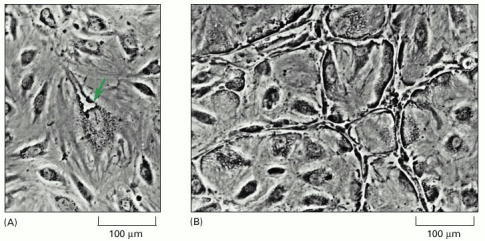
\includegraphics[width=0.6\textwidth]{images/hallowStructureEndothelialCells.jpg}
	\caption{The endothelial cells, when supported by suitable growth medium and signals, start to form hallow structure, that do not contain any blood, and not fluid passes through them. This indicates that the no mechanical trigger (i.e. pressure) is required to form the hallow structure for the new vessels. Image from \cite{Alberts2002}.}
\end{wrapfigure}


	``Experiments in culture show that endothelial cells in a medium containing suitable growth factors will spontaneously form capillary tubes, even if they are isolated from all other types of cells (Figure 22-26). The capillary tubes that develop do not contain blood, and nothing travels through them, indicating that blood flow and pressure are not required for the initiation of a new capillary network. Endothelial cells in culture spontaneously develop internal vacuoles that appear to join up from cell to cell, giving rise to a network of capillary tubes. These photographs show successive stages in the process.''





\section{Biological Assays to Study Angiogenesis}

\subsection{Corneal Micropocket Assay}
This is one of the simple and reproducible assays to study angiogenesis in a eye. The process involves introducing growth factors in the eye ball of mouse, and then letting the vascular network to form. This is a video from JOVE explaining the details of the protocol \citep{conealMicroPocketAssayJOVE} 